\achapter{4}{Vector Representation} \label{sec:vector_representation}

\vspace*{-17 pt}
\framebox{\hspace*{3 pt}
\parbox{4.7 in}{\begin{fqs}
\item What is a vector? 
\item How do we define operations on vectors?
\item What is a linear combination of vectors?
\item How do we determine if one vector is a linear combination of a given set of vectors? 
\item How do we represent a linear system as a vector equation? 
\item What is the span of a set of vectors? 
\item What are possible geometric representations of the span of a vector, or the span of two vectors?
\end{fqs}} \hspace*{3 pt}}

\vspace*{13 pt}

\csection{Application: The Knight's Tour}

Chess is a game played on an $8 \times 8$ grid which utilizes a variety of different pieces. One piece, the knight, is different from the other pieces in that it can jump over other pieces. However, the knight is limited in how far it can move in a given turn. For these reasons, the knight is a powerful, but often under-utilized, piece. 

A knight can move two units either horizontally or vertically, and one unit perpendicular to that. Four knight moves are  as illustrated in Figure \ref{F:knight_1}, and the other four moves are the opposites of these. 
\begin{figure}[h]
\begin{center}
\resizebox{!}{2.5in}{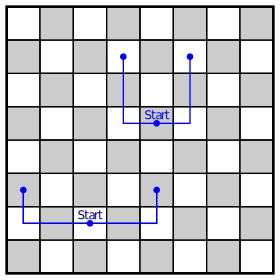
\includegraphics{knight_moves_1}}
\caption{Moves a knight can make.}
\label{F:knight_1}
\end{center}
\end{figure}
%[trim=3cm 0cm 3cm 0cm, clip]

The knight's tour problem is the mathematical problem of finding a knight's tour, that is a sequence of knight moves so the knight visits each square exactly once. While we won't consider a knight's tour in this text, we will see, using linear combinations of vectors, that a knight can move from its initial position to any other position on the board, and that it is possible to determine a sequence of moves to make that happen.

\csection{Introduction}

So far we learned of a convenient method to represent a linear system using matrices. We now consider another representation of a linear system using \emph{vectors}. Vectors can represent concepts in the physical world like velocity, acceleration, and force -- but we will be interested in vectors as algebraic objects in this class. Vectors will form the foundation for everything we will do in linear algebra. For now, the following definition will suffice.

\begin{definition} A (real) \textbf{vector}\index{vector} is a finite list of real numbers in a specified order. Each number in the list is referred to as an \textbf{entry}\index{vector!entry} or \textbf{component}\index{vector!component} of the vector.
\end{definition}

\noindent \textbf{Note}: For the majority of this text, we will work with real vectors. However, A vector does not need to be restricted to have real entries. At times we will use complex vectors and even vectors in other types of sets. The types of sets we use will be ones that have structure just like the real numbers. Recall that a real number is a number that has a decimal representation, either finite or repeating (rational numbers) or otherwise (irrational numbers). We can add and multiply real numbers as we have done throughout our mathematical careers, and the real numbers have a certain structure given in the following theorem that we will treat as an axiom -- that is, we assume these properties without proof. We denote the set of real numbers with the symbol $\R$. 

\begin{theorem} \label{thm:1_d_reals} Let $x$, $y$, and $z$ be real numbers. Then
\begin{itemize}
\item $x + y \in \R$ and $xy \in \R$ (\emph{The name given to this property is closure. That is, the set $\R$ is closed under addition and multiplication.})
\item $x + y = y + x$ and $xy=yx$ (\emph{The name given to this property is commutativity. That is addition and multiplication are commutative operations in $\R$.})
\item $(x + y) + z = x + (y + z)$ and $(xy)z = x(yz)$ (\emph{The name given to this property is associativity. That is, addition and multiplication is associative operations in $\R$.})
\item There is an element $0$ in $\R$ such that $x+ 0 = x$ (\emph{The element $0$ is called the  additive identity in $\R$.}) 
\item There is an element $1$ in $\R$ such that $(1)x = x$ (\emph{The element $1$ is called the  multiplicative identity in $\R$.}) 
\item There is an element $-x$ in $\R$ such that $x+(-x) = 0$ (\emph{The element $-x$ is the additive inverse of $x$ in $\R$.}) 
\item If $x \neq 0$, there is an element $\frac{1}{x}$ in $\R$ such that $x\left(\frac{1}{x}\right) = 1$ (\emph{The element $\frac{1}{x}$ is the multiplicative inverse of the nonzero element $x$ in $\R$.}) 
\item $x (y + z) = (x y) + (x z)$ (\emph{The is the distributive property. That is, multiplication distributes over addition in $\R$.}) 
\end{itemize}
\end{theorem}
Any set that satisfies the properties listed in Theorem  \ref{thm:1_d_reals} is called a \emph{field}\index{field}. We our vectors are made from elements of a field, we call those elements of the field \emph{scalars}\index{scalars}. 


We will algebraically represent a vector as a matrix with one column. For example, $\vv = \left[ \begin{array}{c} 1\\ 2\end{array} \right]$ is a vector with 2 entries, and we say that $\vv$ is a vector in 2-space. By 2-space we mean $\R^2$, which can be geometrically modeled as the plane. Here the symbol $\R$ indicates that the entries of $\vv$ are real numbers and the superscript 2 tells us that $\vv$ has two entries. Similarly, vectors in $\R^3$ have three entries, e.g., $\left[ \begin{array}{r} 1\\ 3\\ -1\end{array} \right]$. The collection of column vectors with three entries can be geometrically modeled as three-dimensional space. If a vector $\vv$ has $n$ entries we say that $\vv$ is a vector in $\R^n$ (or $n$-space). Vectors are also often indicated with arrows, so we might also see a vector $\vv$ written as $\overrightarrow{v}$. It is important when writing to differentiate between a vector $\vv$ and a scalar $v$. These are quite different objects and it is up to us to make sure we are clear what a symbol represents. We will use boldface letters to represent vectors.

A vector like $\left[ \begin{array}{c} 1\\ 2\end{array} \right]$ is called a \emph{column vector}\index{vector!column} of \emph{size} $2 \times 1$ (two rows, one column). We can define an addition operation on two vectors of the same size by adding corresponding components, such as 
\[\left[ \begin{array}{r} 1 \\ -2 \end{array} \right] + \left[ \begin{array}{c} 3 \\ 4 \end{array} \right] = \left[ \begin{array}{c} 4 \\ 2 \end{array} \right].\]


Similarly, we can define scalar multiplication of a vector by multiplying each component of the vector by the scalar. For example,
\[3\left[ \begin{array}{c} 1\\ 2\end{array} \right] = \left[ \begin{array}{c} 3\\ 6\end{array} \right].\]
Since we can add vectors and multiply vectors by scalars, we can then add together scalar multiples of vectors. For completeness, we define vector subtraction as adding a scalar multiple:
\[\vv - \vu = \vv + (-1)\vu.\]
This definition is equivalent to defining subtraction of $\vu$ from $\vv$ by subtracting components of $\vu$ from the corresponding components of $\vv$.

\begin{pa} \label{pa:1_d} ~
\be 
\item Given vectors
\[ \vv =\left[ \begin{array}{r} 1 \\ -2 \\ 2 \end{array} \right] \, , \, \vu=\left[ \begin{array}{c} 0 \\ 1\\ 3 \end{array} \right] \, , \, \vw= \left[ \begin{array}{c} 1\\ 1\\ 4 \end{array} \right]\, , \]
determine the components of the vector $3\vv + \vu - 2\vw$ using the operations defined above.



\begin{comment}
The resulting vector is $\left[ \begin{array}{r} 1 \\ -7 \\ 1 \end{array} \right] $


\end{comment}

\item In mathematics, any time we define operations on objects, such as addition of vectors, we ask which properties the operation has. For example, one might wonder if $\vu+\vv=\vv+\vu$ for any two vectors $\vu, \vv$ of the same size. If this property holds, we say that the \emph{addition of vectors is a commutative operation}. However, to verify this property we cannot use examples since the property must hold for any two vectors. For simplicity, we focus on two-dimensional vectors $\vu = \left[ \begin{array}{c} u_1\\ u_2\end{array} \right]$ and $\vv = \left[ \begin{array}{c} v_1\\ v_2\end{array} \right]$. Using these arbitrary vectors, can we say that $\vu+\vv=\vv+\vu$? If so, justify. If not, give a counterexample. (Note: Giving a counterexample is the best way to justify why a general statement is not true.)


		

\item One way to geometrically represent vectors with two components uses a point in the plane to correspond to a vector. Specifically, the vector $\left[ \begin{array}{c} x \\ y \end{array} \right]$ corresponds to the point $(x, y)$ in the plane. As a specific example, the vector $\left[ \begin{array}{c} 1 \\ 2 \end{array} \right]$ corresponds to the point $(1, 2)$ in the plane. This representation will be especially handy when we consider infinite collections of vectors as we will do in this problem.

\ba
\item On the same set of axes, plot the points that correspond to 5-6 scalar multiples of the vector $\left[ \begin{array}{c} 1 \\ 2 \end{array} \right]$. Make sure to use  variety of scalar multiples covering possibilities with $c>0, c<0, c>1, 0<c<1, -1<c<0$. If we consider the collection of all possible scalar multiples of this vector, what do we obtain?

 

\begin{comment}
This gives us a line through the origin and the point $(1,2)$.



\end{comment}

\item What would the collection of all scalar multiples of the vector $\left[ \begin{array}{c} 0 \\ 0 \end{array} \right]$ form in the plane? 

 

\begin{comment}
We only get the origin.
\end{comment}

\item What would the collection of all scalar multiples of the vector $\left[ \begin{array}{c} 1 \\ 1\\ 1 \end{array} \right]$ form in the three-dimensional space? 



\begin{comment}
This again gives us a line through the origin and the point $(1,1,1)$, but the line is in three-dimensional space.
\end{comment}
\ea

\item Let $\vu=\left[ \begin{array}{c} 1\\ 2 \end{array} \right]$ and $\vv=\left[ \begin{array}{r} 1\\ -1 \end{array} \right]$ in $\R^2$. We are interested in finding all vectors that can be formed as a sum of scalar multiples of $\vu$ and $\vv$.
\ba
\item On the same set of axes, plot the points that correspond to the vectors $\vu, \vv, \vu+\vv, 1.5\vu, 2\vv, -\vu, -\vv, -\vu+2\vv$.  Plot other random sums of scalar multiples of $\vu$ and $\vv$ using several scalar multiples (including those less than 1 or negative) (that is, find other vectors of the form $a\vu + b\vv$ where $a$ and $b$ are any scalars.).


\item If we considered sums of all scalar multiples of $\vu, \vv$, which vectors will we obtain? Can we obtain any vector in $\R^2$ in this form?



\ea


\ee


\end{pa}


\csection{Vectors and Vector Operations}

As discussed in Preview Activity \ref{pa:1_d}, a vector is simply a list of numbers. We can add vectors of like size and multiply vectors by scalars. These operations define a structure on the set of all vectors with the same number of components that will be our major object of study in linear algebra. Ultimately we will expand our idea of vectors to a more general context and study what we will call \emph{vector spaces}.

In Preview Activity \ref{pa:1_d} we saw how to add vectors and multiply vectors by scalars in $\R^2$, and this idea extends to $\R^n$ for any $n$. Before we do so, one thing we didn't address in Preview Activity \ref{pa:1_d}  is what it means for two vectors to be equal. It should seem reasonable that two vectors are equal if and only if they have the same corresponding components. More formally, if we let  
\[\vu = \left[ \begin{array}{c} u_1 \\ u_2 \\ \vdots \\ u_n \end{array} \right] \ \text{ and } \ \vv = \left[ \begin{array}{c} v_1 \\ v_2 \\ \vdots \\ v_n \end{array} \right]\]
be vectors in $\R^n$, then $\vu = \vv$ if $u_i = v_i$ for every $i$ between 1 and $n$. Note that this statement implies that a vector in $\R^2$ cannot equal a vector in $\R^3$ because they don't have the same number of components. With this in mind we can now define the sum $\vu + \vv$ of the vectors $\vu$ and $\vv$ to be the vector in $\R^n$ defined by
\[\vu + \vv = \left[ \begin{array}{c} u_1+v_1 \\ u_2+v_2 \\ \vdots \\ u_n+v_n \end{array} \right].\]
In other words, to add two vectors of the same size, we add corresponding components.

Similarly, we can define scalar multiplication of a vector. If $c$ is a scalar, then the scalar multiple $c \vv$ of the vector $\vv$ is the vector in $\R^n$ defined by
\[c\vv = \left[ \begin{array}{c} cv_1 \\ cv_2 \\ \vdots \\ cv_n \end{array} \right].\]
In other words, the scalar multiple $c\vv$ of the vector $\vv$ is the vector obtained by multiplying each component of the vector $\vv$ by the scalar $c$. Since we can add vectors and multiply vectors by scalars, we can then add together scalar multiples of vectors. For completeness, we define vector subtraction as adding a scalar multiple:
\[\vv - \vu = \vv + (-1)\vu.\]
This definition is equivalent to defining subtraction of $\vu$ from $\vv$ by subtracting components of $\vu$ from the corresponding components of $\vv$. 


After defining operations on objects, we should wonder what kinds of properties these operations have. For example, with the operation of addition of real numbers we know that $1+2$ is equal to $2+1$. This is called the \emph{commutative} property of scalar addition and says that order does not matter when we add real numbers. It is natural for us to ask if similar properties hold for the vector operations, addition and scalar multiplication, we defined. You showed in Preview Activity \ref{pa:1_d} that the addition operation is also commutative on vectors in $\R^2$. 



In the activity below we consider how the two operations, addition and scalar multiplication, interact with each other. In real numbers, we know that multiplication is distributive over addition. Is that true with vectors as well?



\begin{activity} \label{act:A1.3_1} We work with vectors in $\R^2$ to make the notation easier. 
	
Let $a$ be an arbitrary scalar, and $\vu = \left[ \begin{array}{c} u_1\\ u_2\end{array} \right]$ and $\vv = \left[ \begin{array}{c} v_1\\ v_2\end{array} \right]$ be two \emph{arbitrary} vectors in $\R^2$. Is $a(\vu + \vv)$ equal to $a\vu + a\vv$? What property does this imply about the scalar multiplication and addition operations on vectors?



\begin{comment}

We use the fact that $v_1$, $v_2$, $u_1$, and $u_2$ are scalars and addition of scalars is commutative to see that
\[\vv + \vu = \left[ \begin{array}{c} v_1\\ v_2\end{array} \right] + \left[ \begin{array}{c} u_1\\ u_2\end{array} \right] = \left[ \begin{array}{c} v_1+u_1\\ v_2 + u_2 \end{array} \right] = \left[ \begin{array}{c} u_1+v_1 \\ u_2+v_2 \end{array} \right] = \left[ \begin{array}{c} u_1 \\ u_2 \end{array} \right] + \left[ \begin{array}{c} v_1 \\ v_2 \end{array} \right]  = \vu + \vv.\]
So the vector sum is a commutative operation. 

\end{comment}

\end{activity}



Similar arguments can be used to show the following properties of vector addition and multiplication by scalars.



\begin{theorem} \label{thm:vector_properties} Let $\vv$, $\vu$, and $\vw$ be vectors in $\R^n$ and let $a$ and $b$ be scalars. Then
\begin{enumerate}
\item $\vv + \vu = \vu + \vv$
\item $(\vv + \vu) + \vw = \vv + (\vu + \vw)$
\item The vector $\vz = \left[ \begin{array}{c} 0 \\ 0 \\ \vdots \\ 0 \end{array} \right]$ has the property that $\vv + \vz = \vv$. The vector $\vz$ is called the \textbf{zero vector}.
\item  $(-1)\vv + \vv = \vz$. The vector $(-1)\vv = -\vv$ is called the \textbf{additive inverse} of the vector $\vv$.
\item $(a+b) \vv = a\vv + b\vv$
\item $a(\vv + \vu) = a\vv + a\vu$
\item $(ab) \vv = a(b\vv)$
\item $1 \vv = \vv$.
\end{enumerate}
\end{theorem}



We will later see that the above properties make the set $\R^n$ a \emph{vector space}. These properties just say that, for the most part, we can manipulate vectors just as we do real numbers. Please note, though, that there is no multiplication or division of vectors. 

\csection{Geometric Representation of Vectors and Vector Operations}

We can geometrically represent a vector $\vv = \left[ \begin{array}{c} v_1\\ v_2\end{array} \right] $ in $\R^2$ as the point $(v_1, v_2)$ in the plane as we did in Preview Activity \ref{pa:1_d}. We can similarly represent a vector $\vv = \left[ \begin{array}{c} v_1\\ v_2\\ v_3 \end{array} \right]$ in $\R^3$ as the point $(v_1, v_2, v_3)$ in the three-dimensional space. This geometric representation will be handy when we consider collections of infinitely many vectors, as we will do when we consider the span of a collection of vectors later in this section.


We can also represent the vector $\vv = \left[ \begin{array}{c} v_1\\ v_2\end{array} \right] $ in $\R^2$ as the directed line segment (or arrow) from the origin to the point $(v_1, v_2)$ as shown in Figure \ref{F:Vector1} to aid in the visualization. 
\begin{figure}[ht] \centering
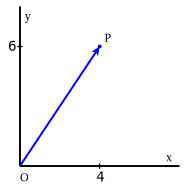
\includegraphics[width=3.7cm]{1_d_a_1}
\caption{The vector~\usebox{\smlmat} in $\R^2$.}
\label{F:Vector1}
\end{figure}

The fact that the vector in Figure \ref{F:Vector1} is represented by the directed line segment from the origin to the point (4,6) means that this vector is the vector $\vv = \left[ \begin{array}{c} 4\\ 6\end{array} \right] $. If $O$ is the origin and $P$ is the point $(4,6)$, we will also denote this vector as $\overrightarrow{OP}$ -- so
\[\overrightarrow{OP} = \left[ \begin{array}{c} 4\\ 6\end{array} \right] .\]
In this way we can think of vectors as having direction and length. With the Pythagorean Theorem, we can see that the length of a vector $\vv = \left[ \begin{array}{c} v_1\\v_2 \end{array} \right]$ is $\sqrt{v_1^2+v_2^2}$. This idea can be applied to vectors in any space. If $\vv = \left[ \begin{array}{c} v_1 \\ v_2 \\ v_3 \\ \vdots \\ \ v_n \end{array} \right]$ is a vector in $\R^n$, then the \textbf{length}\index{vector!length in $\R^n$} of $\vv$, denoted $|\vv|$ is the scalar 
\[||\vv|| = \sqrt{v_1^2+v_2^2+ \cdots + v_n^2}.\]



Thinking of vectors having direction and length is especially useful in visualizing the addition of vectors. The geometric interpretation of the sum of two vectors can be seen in Figures \ref{F:vector_sum_1} and \ref{F:vector_sum_2}.

\begin{figure}[ht]
\begin{center}
\begin{minipage}{1.75in}
\begin{center}
\resizebox{!}{1.5in}{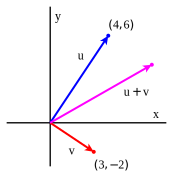
\includegraphics{1_d_a_3}}
\end{center}
\caption{A vector sum.}
\label{F:vector_sum_1}
\end{minipage} \hspace{0.5in}
\begin{minipage}{1.75in}
\begin{center}
\resizebox{!}{1.5in}{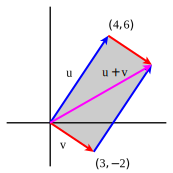
\includegraphics{1_d_a_4}}
\end{center}
\caption{Geometric interpretation.}
\label{F:vector_sum_2}
\end{minipage} 
\end{center}
\end{figure}

Let $\vu = \left[ \begin{array}{c} 4\\ 6\end{array} \right] $ and $\vv = \left[ \begin{array}{r} 3\\ -2\end{array} \right] $. Then $\vu + \vv = \left[ \begin{array}{c} 7\\ 4\end{array} \right] $ as shown in Figure \ref{F:vector_sum_1}. Figure \ref{F:vector_sum_2} provides a context to interpret this vector sum geometrically. Using the parallelogram imposed on the three vectors, we see that if vectors $\vu$ and $\vv$ are both placed to start at the origin, then the vector sum $\vu + \vv$ can be visualized geometrically as the directed line segment from the origin to the fourth corner of the parallelogram.


In Preview Activity \ref{pa:1_d} we considered scalar multiples of a vector in $\R^2$. The arrow representation helps in visualizing scalar multiples as well. Geometrically, a scalar multiple $c\vv$ of a nonzero vector $\vv$ is a vector in the same direction as $\vv$ if $c>0$ and in the opposite direction as $\vv$ if $c<0$. If $c>1$, scalar multiplication stretches the vector, while $0<c<1$ shrinks the vector. We also saw that the collection of all scalar multiples of a vector $\vv$ in $\R^2$ gives us a line through the origin and $\vv$, except when $\vv=\vzero$ in which case we only obtain $\vzero$. In other words, for a nonzero vector $\vv$, the set $S = \{c\vv : c \text{ is a scalar}\}$ is the line through the origin and $\vv$ in $\R^2$. 

All of these properties generalize to vectors in $\R^3$. Specifically, the scalar multiple $c\vv$ is a vector in the same or opposite direction as $\vv$ based on the sign of $c$, and is a stretched or shrunken version of $\vv$ based on whether $|c|>1$ or $|c|<1$. Also, the collection of all multiples of a non-zero vector $\vv$ in $\R^3$ form a line through the origin.

\csection{Linear Combinations of Vectors}

The concept of linear combinations is one of the fundamental ideas in linear algebra. We will use linear combinations to describe almost every important concept in linear algebra -- the span of a set of vectors, the range of a linear transformation, bases, the dimension of a vector space -- to name just a few. 

In Preview Activity \ref{pa:1_d}, we considered the sets of all scalar multiples of a single nonzero vector in $\R^2$ and in $\R^3$. We also considered the set of all sums of scalar multiples of two nonzero vectors. These results so far gives us an idea of geometrical descriptions of sets of vectors generated by one or two vectors. 
Oftentimes we are interested in what vectors can be made from a given collection of vectors. For example, suppose we have two different water-benzene-acetic acid chemical solutions, one with 40\% water, 50\% benzene and 10\% acetic acid, the other with 52\% water, 42\% benzene and 6\% acid. An experiment we want to conduct requires a chemical solution with 43\% water, 48\% benzene and 9\% acid. We would like to know if we make this new chemical solution by mixing the first two chemical solutions, or do we have to run to the chemical solutions market to get the chemical solution we want.

We can set up a system of equations for each ingredient and find the answer. But we can also consider each chemical solution as a vector, where the components represent the water, benzene and acid percentages. So the two chemical solutions we have are represented by the vectors $\vv_1 = \left[ \begin{array}{c} 40\\50\\10\end{array} \right]$ and $\vv_2 = \left[ \begin{array}{c} 52\\42\\6\end{array} \right]$. If we mix the two chemical solutions with varying amounts of each ingredient, then the question of whether we can make the desired chemical solution becomes the question of whether the equation 
\[ c_1\left[ \begin{array}{c} 40\\50\\10\end{array} \right]+ c_2\left[ \begin{array}{c} 52\\42\\6\end{array} \right] = \left[ \begin{array}{c} 43\\48\\9\end{array} \right]\]
has a solution. (You will determine if this equation has a solution in Exercise \ref{ex:1_d_acid}.) 


We might also be interested in what other chemical solutions we can make from the two given solutions. This amounts to determining which vectors can be written in the form $c_1\left[ \begin{array}{c} 40\\50\\10\end{array} \right]+ c_2\left[ \begin{array}{c} 52\\42\\6\end{array} \right]$ for scalars $c_1$ and $c_2$. Vectors that are created from sums of scalar multiples of given vectors are called linear combinations of those vectors. More formally, 

\begin{definition} \label{1_d_linear_combination} A \textbf{linear combination}\index{linear combination} of vectors $\vv_1$, $\vv_2$, $\ldots$, $\vv_m$ in $\R^n$ is any vector of the form
\begin{equation}
c_1 \vv_1 + c_2 \vv_2 + \cdots + c_m \vv_m, \label{eq:lin_comb}
\end{equation}
where $c_1$, $c_2$, $\ldots$, $c_m$ are scalars that we will refer to as the \textbf{weights}\index{linear combination!weights}.
\end{definition}

In the chemical solutions example, the vector $c_1\left[ \begin{array}{c} 40\\50\\10\end{array} \right]+ c_2\left[ \begin{array}{c} 52\\42\\6\end{array} \right]$ for scalars $c_1$ and $c_2$ is a linear combination of the vectors $\left[ \begin{array}{c} 40\\50\\10\end{array} \right]$ and $\left[ \begin{array}{c} 52\\42\\6\end{array} \right]$ with weights $c_1$ and $c_2$, and the set of linear combinations of the given chemical solution vectors tells us exactly which chemical solutions we can make from the given ones. This is one example of how linear combinations can arise in applications.  

The set of all linear combinations of a fixed collection of vectors has a very nice algebraic structure and, in small dimensions, allows us to use a geometrical description to aid our understanding. In the above example, this collection gives us the type of chemical solutions we can make by combining the first two solutions in varying amounts. 

\begin{activity} \label{act:A1.3_7} %Let $\vv_1 = \left[ \begin{array}{c} 1 \\ 1 \\ 1 \end{array} \right]$ and $\vv_2 = \left[ \begin{array}{r} 2 \\ -1 \\ 3 \end{array} \right]$. 
Our chemical solution example illustrates that it can be of interest to determine whether certain vectors can be written as a linear combination of given vectors. We explore that idea in more depth in this activity. Let $\vv_1=\left[ \begin{array}{c} 1 \\ 1 \\ 1 \end{array} \right]$ and $\vv_2=\left[ \begin{array}{r} 2 \\ -1 \\ 3 \end{array} \right]$.  

    \ba
    \item Calculate the linear combination of $\vv_1$ and $\vv_2$ with corresponding weights (scalar multiples) 1 and 2. The resulting vector is a vector which can be written as a linear combination of $\vv_1$ and $\vv_2$.

    
		
		\item Can $\vw = \left[ \begin{array}{c} 3 \\ 0 \\ 4 \end{array} \right]$ be written as a linear combination of $\vv_1$ and $\vv_2$? If so, which linear combination? If not, explain why not.
		
		

    \item Can $\vw = \left[ \begin{array}{c} 2 \\ 0 \\ 2 \end{array} \right]$ be written as a linear combination of $\vv_1$ and $\vv_2$? If so, which linear combination? If not, explain why not.
		
		

    \item Let $\vw = \left[ \begin{array}{r} 0 \\ 6 \\ -2 \end{array} \right]$. The problem of determining if $\vw$ is a linear combination of $\vv_1$ and $\vv_2$ is equivalent to the problem of finding scalars $x_1$ and $x_2$ so that
    \begin{equation}
    \vw = x_1 \vv_1 + x_2 \vv_2 . \label{eq:vect_eq1}
    \end{equation}
		\begin{enumerate}[i.]
		\item Combine the vectors on the right hand side of equation (\ref{eq:vect_eq1}) into one vector, and then set the components of the vectors on both sides equal to each other to convert the vector equation (\ref{eq:vect_eq1}) to a linear system of three equations in two variables.


		\item Use row operations to find a solution, if it exists, to the system you found in the previous part of this activity. If you find a solution, verify in (\ref{eq:vect_eq1}) that you have found appropriate weights to produce the vector $\vw$ as a linear combination of $\vv_1$ and $\vv_2$.


		\end{enumerate}
		
    \ea
\end{activity}



Note that to find the weights that make $\vw$ a linear combination of the vectors $\vv_1$ and $\vv_2$, we simply solved the linear system corresponding to the augmented matrix
\[[\vv_1 \  \vv_2 \ | \ \vw],\]
where the vectors $\vv_1$, $\vv_2$, and $\vw$ form the columns of an augmented matrix, and the solution of the system gave us the weights of the linear combination. In general, if we want to find weights $c_1$, $c_2$, $\ldots$, $c_m$ so that a vector $\vw$ in $\R^n$ is a linear combination of the vectors $\vv_1$, $\vv_2$, $\ldots$, $\vv_m$ in $\R^n$, we solve the system corresponding to the augmented matrix
\[[\vv_1 \  \vv_2 \  \vv_3 \ \cdots \ \vv_m | \ \vw].\]
Any solution to this system will gives us the weights. If this system has no solutions, then $\vw$ cannot be written as a linear combination of the vectors $\vv_1$, $\vv_2$, $\ldots$, $\vv_m$. This shows us the equivalence of the linear system and its vector equation representation. Specifically, we have the following result.


\begin{theorem}
The vector equation
\[x_1 \vv_1 + x_2\vv_2 + x_3\vv_3 + \cdots + x_m\vv_m = \vw\]
has the same solution set as the linear system represented by the augmented matrix
\[[\vv_1 \  \vv_2 \  \vv_3 \ \cdots \ \vv_m | \ \vw].\]
In particular, the system has a solution if and only if $\vw$ is a linear combination of the vectors $\vv_1, \vv_2, \vv_3, \ldots, \vv_m$.
\end{theorem}

\begin{activity} \label{act:A1.3_8} ~
	\ba
	\item Represent the following linear system as a vector equation. After finding the vector equation, compare your vector equation to the matrix representation you found in Preview Activity \ref{pa:1_d}. (Note that this is the same linear system from Preview Activity \ref{pa:1_c}.) 
\begin{equation*}
\begin{split}
-x_3 + 3 + 2x_2&= -x_1   \\
-3 + 2x_3 &= -x_2  \\
-2x_2 + x_1 &= 3x_3-7 
\end{split} 
\end{equation*} 

\begin{comment}
The resulting vector equation is
\[x_1 \left[ \begin{array}{r} 1 \\0 \\-1 \end{array} \right] +x_2 \left[ \begin{array}{r} 2 \\ 1\\ -2 \end{array} \right] + x_3 \left[ \begin{array}{r} -1 \\ 2 \\ -3 \end{array} \right] = \left[ \begin{array}{r} -3 \\ 3\\ -7\end{array} \right]  \]
The vectors are the columns of the augmented matrix representation.


\end{comment}

	\item Represent the following vector equation as a linear system and solve the linear system.
\[x_1 \left[ \begin{array}{c} 1 \\ 1 \\ 2 \end{array} \right] +x_2 \left[ \begin{array}{c} 1 \\ 2\\ 3 \end{array} \right] + x_3 \left[ \begin{array}{r} -1 \\ 2 \\ -3 \end{array} \right] = \left[ \begin{array}{c} 4 \\ 3\\ 11 \end{array} \right] \]


\begin{comment}

This system is the same as the system in the second problem of Preview Activity \ref{pa:1_b}.

\end{comment}

	\ea
\end{activity}


\csection{The Span of a Set of Vectors}

As we saw in the previous section, the question of whether a system of linear equations has a solution is equivalent to the question of whether the vector obtained by the non-coefficient constants in the system is a linear combination of the vectors obtained from the columns of the coefficient matrix of the system. So if we were interested in finding for which constants the system has a solution, we would look for the collection of all linear combinations of the columns. We call this collection the \emph{span} of these vectors. In this section we investigate the concept of span both algebraically and geometrically.

Our work in Preview Activity \ref{pa:1_d} seems to indicate that the span of a set of vectors, i.e., the collection of all linear combinations of this set of vectors, has a nice structure. As we mentioned above, the span of a set of vectors represents the collection of all constant vectors for which a linear system has a solution, but we will also see that other important objects in linear algebra can be represented as the span of a set of vectors.



\begin{definition} \label{def:1_d_span}  The \textbf{span}\index{span} of the vectors $\vv_1$, $\vv_2$, $\ldots$, $\vv_m$ in $\R^n$ is the collection of all  linear combinations of the vectors $\vv_1$, $\vv_2$, $\ldots$, $\vv_m$.
\end{definition}



\noindent \textbf{Notation:} We denote the span of a set of vectors $\vv_1$, $\vv_2$, $\ldots$, $\vv_m$ as
\[\Span \{\vv_1, \vv_2, \ldots, \vv_m\} .\]
So
\[\Span \{\vv_1, \vv_2, \ldots, \vv_m\}  = \{c_1\vv_1+c_2\vv_2 + \cdots + c_m \vv_m : c_1, c_2, \ldots, c_m \text{ are scalars}\}.\]
The curly braces, $\{ \; \}$, are used in denoting sets. They represent the whole set formed by the objects included between them. So $\{\vv_1, \vv_2, \ldots, \vv_m\}$ represents the collection of the vectors formed by $\vv_1, \vv_2, \ldots, \vv_m$ for an arbitrary number $m$. Note that $m$ can be 1, meaning that the collection can contain only one vector $\vv_1$.



We now investigate what the span of a set of one or two vectors is, both from an algebraic and geometric perspective, and consider what happens for more general spanning sets.

\begin{activity} \label{act:A1.3_9} ~
	\ba
	\item By definition, $\Span\left\{\left[ \begin{array}{r} 1 \\ -2 \end{array} \right]\right\}$ is the collection of all vectors which are scalar multiples of $\left[ \begin{array}{r} 1 \\ -2 \end{array} \right]$. Determine which vectors are in this collection. If we plot all these vectors with each vector being represented as a point in the plane, what do they form?


	\item Let $\vv_1 = \left[ \begin{array}{c} 1 \\ 0\\ 1 \end{array} \right]$ and $\vv_2 = \left[ \begin{array}{c} 0\\1 \\1  \end{array} \right]$ in $\R^3$. By definition, 
\[\Span\left\{\left[ \begin{array}{c} 1 \\ 0\\ 1 \end{array} \right], \left[ \begin{array}{c} 0\\1 \\1  \end{array} \right] \right\}\]
 is the collection of all linear combinations of the form 
\[x_1 \left[ \begin{array}{c} 1 \\ 0\\ 1 \end{array} \right] + x_2 \left[ \begin{array}{c} 0\\1 \\1  \end{array} \right],\]
where $x_1$ and $x_2$ are any scalars. 
		\begin{enumerate}[i.]
		\item Find four different vectors in $\Span \{\vv_1, \vv_2\} $ and indicate the weights (the values of $x_1$ and $x_2$) for each linear combination. (Hint: It is really easy to find 3 vectors in $\Span \{\vv_1, \vv_2\} $ for any $\vv_1, \vv_2$.)

        

		\item Are there any vectors in $\R^3$ that are not in $\Span\{\vv_1, \vv_2\}$? Explain. Verify your result.



		\item Set up a linear system to determine which vectors $\vw= \left[ \begin{array}{c} w_1 \\ w_2\\ w_3 \end{array} \right]$ are in $\Span\{\vv_1, \vv_2\}$. Specifically, which $\vw$ can be expressed as a linear combination of $\vv_1$ and $\vv_2$?

    
		
		\item Geometrically, what shape do the vectors in $\Span\{\vv_1, \vv_2\}$ form inside $\R^3$?
		
		\end{enumerate}
		

\item Is it possible for $\Span\{\vz_1, \vz_2\}$ to be a line for two vectors $\vz_1, \vz_2$ in $\R^3$?
		
	
    \item What do you think are the possible geometric descriptions of a span of a set of vectors in $\R^2$? Explain.

    

    \item What do you think are the possible spans of a set of vectors in $\R^3$? Explain.

    

    \ea
\end{activity}


\csection{Examples}

\ExampleIntro

\begin{example} For each of the following systems, 
	\begin{itemize}
	\item express an arbitrary solution to the system algebraically as a linear combination of vectors,
	\item find a set of vectors that spans the solution set,
	\item describe the solution set geometrically.
	\end{itemize}
\ba
\item ~
\begin{alignat*}{5}
{}x_1 	&{}{} 		&{} 		&{}+{}		&{}x_3 		&= &{} 	&0&{} \\
{2}x_1 	&{}+{}	&{}x_2 	&{}+{} 		&{3}x_3 		&= &{} 	&0&{} \\
{4}x_1	&{}-{} 	&{}x_2 	&{}+{} 		&{3}x_3		&= &{} 	&0&{.} 
\end{alignat*}
\item ~
\begin{alignat*}{5}
{}x_1 	&{}+{} 	&{2}x_2 	&{}+{}		&{3}x_3 		&= &{} 	&0&{} \\
{2}x_1 	&{}+{}	&{4}x_2 	&{}+{} 		&{6}x_3 		&= &{} 	&0&{} \\
{4}x_1	&{}+{} 	&{8}x_2 	&{}+{} 		&{12}x_3		&= &{} 	&0&{.} 
\end{alignat*}
\ea

\ExampleSolution In each example, we use technology to find the reduced row echelon form of the augmented matrix.
\ba
\item The reduced row echelon form of the augmented matrix
\[\left[ \begin{array}{crc|c} 1&0&1&0 \\ 2&1&3&0 \\ 4&-1&3&0 \end{array} \right]\]
is
\[\left[ \begin{array}{ccc|c} 1&0&1&0 \\ 0&1&1&0 \\ 0&0&0&0 \end{array} \right].\]
	\begin{itemize}
	\item There is no pivot in the $x_3$ column, so $x_3$ is a free variable. Since the system is consistent, it has infinitely many solutions. We can write both $x_1$ and $x_2$ in terms of $x_3$ as $x_2 = -x_3$ and $x_1 = -x_3$. So the general solution to the system has the algebraic form
\[\left[ \begin{array}{c} x_1\\x_2\\x_3 \end{array} \right] = \left[ \begin{array}{r} -x_3\\-x_3\\x_3 \end{array} \right] = x_3\left[ \begin{array}{r} -1\\-1\\1 \end{array} \right].\]
So every solution to this system is a scalar multiple (linear combination) of the vector $\left[ \begin{array}{r} -1\\-1\\1 \end{array} \right]$.
	\item Since every solution to the system is a scalar multiple of the vector $\left[ \begin{array}{r} -1\\-1\\1 \end{array} \right]$, the solution set to the system is $\Span\left\{\left[ \begin{array}{r} -1\\-1\\1 \end{array} \right]\right\}$. 
	\item As the set of scalar multiples of a single vector, the solution set to this system is a line in $\R^3$  through the origin and the point $(-1,-1,1)$. 
	\end{itemize} 
	
\item The reduced row echelon form of the augmented matrix
\[\left[ \begin{array}{ccc|c} 1&2&3&0 \\ 2&4&6&0 \\ 4&8&12&0 \end{array} \right]\]
is
\[\left[ \begin{array}{ccc|c} 1&2&3&0 \\ 0&0&0&0 \\ 0&0&0&0 \end{array} \right].\]
	\begin{itemize}
	\item There are no pivots in the $x_2$ and $x_3$ columns, so $x_2$ and $x_3$ are free variables. Since the system is consistent, it has infinitely many solutions. We can write $x_1$  in terms of  $x_2$ and $x_3$ as $x_1 = -2x_2-3x_3$. So the general solution to the system has the algebraic form
\[\left[ \begin{array}{c} x_1\\x_2\\x_3 \end{array} \right] = \left[ \begin{array}{c} -2x_2-3x_3\\x_2\\x_3 \end{array} \right] = x_2\left[ \begin{array}{r} -2\\1\\0 \end{array} \right] + x_3\left[ \begin{array}{r} -3\\0\\1 \end{array} \right].\]
So every solution to this system is a linear combination of the vectors $\left[ \begin{array}{r} -2\\1\\0 \end{array} \right] $ and $\left[ \begin{array}{r} -3\\0\\1 \end{array} \right]$.
	\item Since every solution to the system is a linear combination of the vectors $\left[ \begin{array}{r} -2\\1\\0 \end{array} \right]$ and $\left[ \begin{array}{r} -3\\0\\1 \end{array} \right]$, the solution set to the system is 
	\[\Span\left\{\left[ \begin{array}{r} -2\\1\\0 \end{array} \right], \left[ \begin{array}{r} -3\\0\\1 \end{array} \right] \right\}.\] 
	\item As the set of linear combinations of two vectors, the solution set to this system is a plane in $\R^3$  through the origin and the points $(-2,1,0)$ and $(-3,0,1)$. 
	\end{itemize} 
\ea
\end{example}

\begin{example} \label{example:1_d_span} Let $W = \left\{\left[ \begin{array}{c} s+t \\ r+2s \\ r-3t \\ r+s+t \end{array} \right] : r,s,t \in \R \right\}$. 
	\ba
	\item Find three vectors $\vv_1$, $\vv_2$, and $\vv_3$ such that $W = \Span\{\vv_1, \vv_2, \vv_3\}$. 
	\item Can $\vw = \left[ \begin{array}{r} -2\\-4\\-1\\0 \end{array} \right]$ be written as a linear combination of the vectors $\vv_1$, $\vv_2$, $\vv_3$? If so, find such a linear combination. If not, justify your response. What does your result tell us about the relationship between $\vw$ and $W$? Explain. 
	\item  Can $\vu = \left[ \begin{array}{r} 3\\-4\\1\\-1 \end{array} \right]$ be written as a linear combination of the vectors $\vv_1$, $\vv_2$, $\vv_3$? If so, find such a linear combination. If not, justify your response. What does your result tell us about the relationship between $\vw$ and $W$? Explain.
	\item What relationship, if any, exists between $\Span\{\vv_1, \vv_2, \vv_3\}$ and $\Span \ W$? Explain. 
	\ea

\ExampleSolution 
\ba
\item Every vector in $W$ has the form
\begin{align*}
\left[ \begin{array}{c} s+t \\ r+2s \\ r-3t \\ r+s+t \end{array} \right] &= \left[ \begin{array}{c} 0 \\ r \\ r \\ r\end{array} \right] + \left[ \begin{array}{c} s \\ 2s \\ 0 \\ s \end{array} \right] + \left[ \begin{array}{r} t \\ 0 \\ -3t \\ t \end{array} \right] \\
	&= r\left[ \begin{array}{c} 0 \\ 1 \\ 1 \\ 1 \end{array} \right] + s\left[ \begin{array}{r} 1 \\ 2 \\ 0 \\ 1 \end{array} \right] + t\left[ \begin{array}{r} 1 \\ 0 \\ -3 \\ 1 \end{array} \right]
\end{align*}
for some real numbers $r$, $s$, and $t$. Thus, $W = \Span\{\vv_1, \vv_2, \vv_3\}$ where $\vv_1 = \left[ \begin{array}{c} 0 \\ 1 \\ 1 \\ 1 \end{array} \right]$, $\vv_2 = \left[ \begin{array}{r} 1 \\ 2 \\ 0 \\ 1 \end{array} \right]$, and $\vv_3 = \left[ \begin{array}{r} 1 \\ 0 \\ -3 \\ 1 \end{array} \right]$. 

\item To determine if $\vw$ is a linear combination of $\vv_1$, $\vv_2$, and $\vv_3$, we row reduced the augmented matrix $[\vv_1 \ \vv_2 \ \vv_3 \ | \ \vw]$. The reduced row echelon form of the matrix $[\vv_1 \ \vv_2 \ \vv_3 \ | \ \vw]$ is
\[\left[ \begin{array}{ccc|r} 1&0&0&2 \\ 0&1&0&-3\\ 0&0&1&1 \\ 0&0&0&0 \end{array}\right].\]
The system with this as augmented matrix is consistent. If we let $x_1$, $x_2$, and $x_3$ be the variables corresponding to the first three columns, respectively, of this augmented matrix, then we see that $x_1 = 2$, $x_2 = -3$, and $x_3 = 1$. So $\vw$ can be written as a linear combination of $\vv_1$, $\vv_2$, and $\vv_3$ as 
\[\vw = 2\vv_1 -3\vv_2 + \vv_3.\]
Since $W = \Span\{\vv_1, \vv_2, \vv_3\}$, it follows that $\vw \in W$. 

\item To determine if $\vu$ is a linear combination of $\vv_1$, $\vv_2$, and $\vv_3$, we row reduced the augmented matrix $[\vv_1 \ \vv_2 \ \vv_3 \ | \ \vu]$. The reduced row echelon form of the matrix $[\vv_1 \ \vv_2 \ \vv_3 \ | \ \vu]$ is
\[\left[ \begin{array}{ccc|c} 1&0&0&0 \\ 0&1&0&0\\ 0&0&1&0 \\ 0&0&0&1 \end{array}\right].\]
The last row shows that the system with this as augmented matrix is inconsistent. So $\vu$ cannot be written as a linear combination of $\vv_1$, $\vv_2$, and $\vv_3$. Since $W = \Span\{\vv_1, \vv_2, \vv_3\}$, it follows that $\vu \not\in W$. 

\item We know that $\Span\{\vv_1, \vv_2, \vv_3\} = W$. Now $\Span \ W$ contains the linear combinations of vectors in $W$, which are all linear combinations of the vectors $\vv_1$, $\vv_2$, and $\vv_3$. Thus, $\Span \ W$ is just the set of linear combinations of $\vv_1$, $\vv_2$, and $\vv_3$. We conclude that  $\Span \ W = \Span\{\vv_1, \vv_2, \vv_3\} = W$. 

\ea

\end{example}

\csection{Summary}

\begin{itemize}
\item A vector is a list of numbers in a specified order. 
\item We add two vectors of the same size by adding corresponding components. In other words, if $\vu$ and $\vv$ are vectors of the same size and $u_i$ and $v_i$ are the $i$ components of $\vu$ and $\vv$, respectively, then $\vu +\vv$ is the vector whose $i$th component is $u_i+v_i$ for each $i$. Geometrically, we represent the sum of two vectors using the Parallelogram Rule: The vector $\vu+\vv$ is the directed line segment from the origin to the 4th point of the parallelogram formed by the origin and the vectors $\vu, \vv$.
\item A scalar multiple of a vector is found by multiplying each component of the vector by that scalar. In other words, if $v_i$ is the $i$ component of the vector $\vv$ and $c$ is any scalar, then $c\vv$ is the vector whose $i$ component is $cv_i$ for each $i$. Geometrically, a scalar multiple of a nonzero vector $\vv$ is a vector in the same direction as $\vv$ if $c>0$ and in the opposite direction if $c<0$. If $|c|>1$, the vector is stretched, and if $|c|<1$, the vector is shrunk.
\item An important concept is that of a linear combination of vectors. In words, a linear combination of a collection of vectors is a sum of scalar multiples of the vectors. More formally, we defined a linear combination of vectors $\vv_1$, $\vv_2$, $\ldots$, $\vv_m$ in $\R^n$ is any vector of the form $c_1 \vv_1 + c_2 \vv_2 + \cdots + c_m \vv_m$, where $c_1$, $c_2$, $\ldots$, $c_m$ are scalars.
\item To find weights $c_1$, $c_2$, $\ldots$, $c_m$ so that a vector $\vw$ in $\R^n$ is a linear combination of the vectors $\vv_1$, $\vv_2$, $\ldots$, $\vv_m$ in $\R^n$, we simply solve the system corresponding to the augmented matrix
\[[\vv_1 \  \vv_2 \  \vv_3 \ \cdots \ \vv_m | \ \vw].\]
\item The collection of all linear combinations of a set of vectors is called the span of the set of vectors. More formally, the span of the vectors $\vv_1$, $\vv_2$, $\ldots$, $\vv_m$ in $\R^n$ is the set
\[\{c_1\vv_1 + c_2\vv_2 + \cdots + c_m\vv_m : c_1, c_2, \ldots, c_m \text{ are scalars}\},\]
which we denote as $\Span \{\vv_1, \vv_2, \ldots, \vv_m\}$. 
Geometrically, the span of a single nonzero vector $\vv$ in any dimension is the line through the origin and the vector $\vv$. The span of two vectors $\vv_1, \vv_2$ in any dimension neither of which is a multiple of the other is a plane through the origin containing both vectors.
\end{itemize}




\csection{Exercises}

\be
\item Given vectors $\vu=\left[ \begin{array}{c} 1 \\ 2 \end{array} \right] $ and $\vv=\left[ \begin{array}{r} -1 \\ 2 \end{array} \right]$ in $\R^2$, determine if $\vw=\left[ \begin{array}{r} -4 \\ -1 \end{array} \right]$ can be written as a linear combination of $\vu$ and $\vv$. If so, determine the weights of $\vu$ and $\vv$ which produce $\vw$.

\item Given vectors $\vv_1=\left[ \begin{array}{c} 1 \\ 2 \\1 \end{array} \right]$, $\vv_2=\left[ \begin{array}{r} -2 \\ 1 \\2 \end{array} \right]$ and $\vv_3=\left[ \begin{array}{r} -1 \\ 3\\3 \end{array} \right]$ in $\R^3$, determine if $\vw=\left[ \begin{array}{c} 5\\ 5\\ 1 \end{array} \right]$ can be written as a linear combination of $\vv_1$, $\vv_2$ and $\vv_3$. If so, determine the weights of $\vv_1$, $\vv_2$ and $\vv_3$ which produce $\vw$. Reflect on the result. Is there anything special about the given vectors $\vv_1$, $\vv_2$ and $\vv_3$?

\item Let $\vu=\left[ \begin{array}{c} 1 \\ 2 \\1  \end{array} \right] $ and $\vv=\left[ \begin{array}{r} -1 \\ 1 \\ 1 \end{array} \right]$ in $\R^3$. Determine which vectors $\vw= \left[ \begin{array}{c} w_1 \\ w_2 \\ w_3 \end{array} \right] $ in $\R^3$ can be written as a linear combination of $\vu$ and $\vv$. Does the set of $\vw$'s include the 0 vector? If so, determine which weights in the linear combination produce the 0 vector. If not, explain why not.


\item Consider vectors $\vu=\left[ \begin{array}{c} 0\\ 2\\0 \end{array} \right]$ and $\vv=\left[ \begin{array}{c} 1\\ 1\\1 \end{array} \right]$ in $\R^3$. 
	\ba
	\item Find four specific linear combinations of the vectors $\vu$ and $\vv$.
	\item Explain why the zero vector must be a linear combination of $\vu$ and $\vv$. 
	\item What kind of geometric shape does the set of all linear combinations of $\vu$ and $\vv$ have in $\R^3$? 
	\item Can we obtain any vector in $\R^3$ as a linear combination of $\vu$ and $\vv$? Explain.
	\ea

\item \label{ex:1_d_acid} Suppose we have two different water-benzene-acetic acid solutions, one with 40\% water, 50\% benzene and 10\% acetic acid, the other with 52\% water, 42\% benzene and 6\% acid. 
	\ba
	\item An experiment we want to conduct requires a solution with 43\% water, 48\% benzene and 9\% acid. Representing each acid solution as a vector, determine if we can we make this new acid solution by mixing the first two solutions, or do we have to run to the chemical solutions market to get the solution we want?
	\item Using the water-benzene-acetic acid solutions in the previous problem, can we obtain an acid solution which contains 50\% water, 43\% benzene and 7\% acid?
	\item Determine the relationship between the percentages of water, benzene, and acid in solutions which can be obtained by mixing the two given water-benzene-acetic acid solutions above. 
	\ea
	
%\item Alka-seltzer contains sodium bicarbonate (NaHCO$_3$) and citric acid (C$_6$H$_8$O$_7$). When a tablet is dissolved in water, the following reaction produces sodium citrate, water and carbon dioxide.
%\begin{center} $x_1$NaHCO$_3$ + $x_2$C$_6$H$_8$O$_7 \rightarrow x_3$Na$_3$C$_6$H$_5$O$_7$ + $x_4$H$_2$O + $x_5$CO$_2$
%\end{center}
%where the number of each molecule on either side of the equation is unknown.
%	\ba
%	\item For each molecule in the above reaction create a vector with entries corresponding to the number of sodium (Na) atoms, carbon (C) atoms, hydrogen (H) atoms, and oxygen (O) atoms (respectively). For example, the vector corresponding to NaHCO$_3$ is $ \left[ \begin{array}{c} 1 \\ 1\\ 1\\ 3 \end{array} \right]$.
%	\item Set up a vector equation that uses the vectors you created above using the law of conservation of mass, i.e. the atoms entering the reaction should equal those coming out. Solve your equation to balance the chemical equation.
%	\ea


\item Is the vector $\vb = \left[ \begin{array}{c} 0\\1\\2 \end{array} \right]$ in $\Span\left\{ \left[ \begin{array}{r} 2\\-1\\0 \end{array} \right], \left[ \begin{array}{r} -3\\0\\-5 \end{array} \right], \left[ \begin{array}{c} 1\\1\\0 \end{array} \right] \right\}$? Justify your answer. 

\item Describe geometrically each of the following sets.
	\ba
	\item $\Span\left\{\left[ \begin{array}{c} 1\\1 \end{array} \right], \left[ \begin{array}{r} -1\\-1 \end{array} \right]\right\}$ in $\R^2$
	\item $\Span\left\{\left[ \begin{array}{c} 1\\1\\1 \end{array} \right], \left[ \begin{array}{r} -1\\-1\\-1 \end{array} \right], \left[ \begin{array}{c} 2\\0\\1 \end{array} \right]\right\}$ in $\R^3$
	\ea

\item Consider the linear system 
\begin{alignat*}{5}
{2}x_1	&{}+{}	&{3}x_2 &{}+{}	&{3}x_3	&{}		&{}		&{}={} &0&{}   \\
{4}x_1	&{}		&{} 		&{}+{}	&{6}x_3	&{}+{}	&{6}x_4	&{}={} &0&{} \\
{2}x_1	&{}+{}	&{4}x_2	&{}+{}	&{3}x_3	&{}-{}	&{}x_4	&{}={} &0&{.} 
\end{alignat*}
	\ba
	\item Find the general solution to this system.
	\item Find two specific vectors $\vv_1$ and $\vv_2$ so that the solution set to this system is $\Span\{\vv_1, \vv_2\}$. 
	\ea
	
\item Answer the following question as yes or no. Verify your answer. If $\vu$ and $\vv$ are vectors in $\R^n$, then $\vv$ is in $\Span\{\vu, \vu-\vv\}$. 



\item Let $\vv$, $\vu$, and $\vw$ be vectors in $\R^n$ and let $a$ and $b$ be scalars. Verify Theorem \ref{thm:vector_properties}. That is, show that 
	\ba
	\item $\vv + \vu = \vu + \vv$
	\item $(\vv + \vu) + \vw = \vv + (\vu + \vw)$
	\item The vector $\vz = \left[ \begin{array}{c} 0 \\ 0 \\ \vdots \\ 0 \end{array} \right]$ has the property that $\vv + \vz = \vv$. 
	\item  $(-1)\vv + \vv = \vz$. 
	\item $(a+b) \vv = a\vv + b\vv$
	\item $a(\vv + \vu) = a\vv + a\vu$
	\item $(ab) \vv = a(b\vv)$
	\item $1 \vv = \vv$.
	\ea

\begin{comment}

Let $\vu = \left[ \begin{array}{c} u_1 \\ u_2 \\ \vdots \\ u_n \end{array} \right]$, $\vv = \left[ \begin{array}{c} v_1 \\ v_2 \\ \vdots \\ v_n \end{array} \right]$, and $\vw = \left[ \begin{array}{c} w_1 \\ w_2 \\ \vdots \\ w_n \end{array} \right]$.
\ba
\item Since addition of real number is commutative, we have 
\begin{align*}
\vv + \vu &= \left[ \begin{array}{c} v_1+u_1 \\ v_2+u_2 \\ \vdots \\ v_n+u_n \end{array} \right] \\
	&= \left[ \begin{array}{c} u_1+v_1 \\ u_2+v_2 \\ \vdots \\ u_n+v_n \end{array} \right] \\
	&= \vu+\vv.
\end{align*}
\item Since addition of real numbers is commutative, we have 
\begin{align*}
(\vv + \vu) +\vw  &= \left(\left[ \begin{array}{c} v_1+u_1 \\ v_2+u_2 \\ \vdots \\ v_n+u_n \end{array} \right] \right) +  \left[ \begin{array}{c} w_1 \\ w_2 \\ \vdots \\ w_n \end{array} \right] \\
	&= \left[ \begin{array}{c} (v_1+u_1)+w_1 \\ (v_2+u_2)+w_2 \\ \vdots \\ (v_n+u_n)+w_n \end{array} \right] \\
	&= \left[ \begin{array}{c} v_1+(u_1+w_1) \\ v_2+(u_2+w_2) \\ \vdots \\ v_n+(u_n+w_n) \end{array} \right] \\
	&= \left[ \begin{array}{c} v_1 \\ v_2 \\ \vdots \\ v_n\end{array} \right] + \left(\left[ \begin{array}{c} (u_1+w_1) \\ (u_2+w_2) \\ \vdots \\ (u_n+w_n) \end{array} \right] \right) \\
	&= \vv + (\vu + \vw).
\end{align*}
\item Note that 
\begin{align*}
\vv + \vz &= \left[ \begin{array}{c} v_1+0 \\ v_2+0 \\ \vdots \\ v_n+0 \end{array} \right] \\
	&= \left[ \begin{array}{c} v_1 \\ v_2 \\ \vdots \\ v_n \end{array} \right] \\
	&= \vv.
\end{align*}
\item By definition of a scalar multiple of a vector and the vector sum,
\begin{ailgn*}
(-1)\vv + \vv &=  \left[ \begin{array}{c} -v_1 \\ -v_2 \\ \vdots \\ -v_n \end{array} \right] +  \left[ \begin{array}{c} v_1 \\ v_2 \\ \vdots \\ v_n \end{array} \right]  \\
	&=  \left[ \begin{array}{c} (-v_1)+v_1 \\ (-v_2)+v_2 \\ \vdots \\ (-v_n)+v_n \end{array} \right]  \\
	&= \left[ \begin{array}{c} 0 \\ 0 \\ \vdots \\ 0 \end{array} \right] \\
	&= \vz.
\end{align*}
\item By definition of a scalar multiple of a vector and the vector sum,
\begin{ailgn*}
(a+b) \vv &=  \left[ \begin{array}{c} (a+b)v_1 \\ (a+b)v_2 \\ \vdots \\ (a+b)v_n \end{array} \right]   \\
	&=  \left[ \begin{array}{c} av_1+bv_1 \\ av_2+bv_2 \\ \vdots \\ av_n+bv_n \end{array} \right]  \\
	&= \left[ \begin{array}{c} av_1 \\ av_2 \\ \vdots \\ av_n \end{array} \right]  + \left[ \begin{array}{c} bv_1 \\ bv_2 \\ \vdots \\ bv_n \end{array} \right]  \\
	&= a\vv + b\vv.
\end{align*}
\item By definition of a scalar multiple of a vector and the vector sum,
\begin{ailgn*}
a\vv + a\vu &=  \left[ \begin{array}{c} av_1 \\ av_2 \\ \vdots \\ av_n \end{array} \right]  + \left[ \begin{array}{c} au_1 \\ au_2 \\ \vdots \\ au_n \end{array} \right]  \\
	&= \left[ \begin{array}{c} av_1+au_1 \\ av_2+au_2 \\ \vdots \\ av_n+au_n \end{array} \right]  \\
	&= \left[ \begin{array}{c} a(v_1+u_1) \\ a(v_2+u_2) \\ \vdots \\ a(v_n+u_n) \end{array} \right]  \\
	&= a\left[ \begin{array}{c} v_1+u_1 \\ v_2+u_2 \\ \vdots \\ v_n+u_n \end{array} \right]  \\
	&= a(\vv + \vu).
\end{align*}
\item By definition of a scalar multiple of a vector and the vector sum,
\begin{ailgn*}
(ab)\vv &=  \left[ \begin{array}{c} (ab)v_1 \\ (ab)v_2 \\ \vdots \\ (ab)v_n \end{array} \right]    \\
	&=  \left[ \begin{array}{c} a(bv_1) \\ a(bv_2) \\ \vdots \\ a(bv_n) \end{array} \right]    \\
	&= a\left[ \begin{array}{c} bv_1 \\ bv_2 \\ \vdots \\ bv_n \end{array} \right]    \\
	&= a(b\vv).
\end{align*}
\item By definition of a scalar multiple of a vector,
\begin{ailgn*}
1\vv &=  \left[ \begin{array}{c} (1)v_1 \\ (1)v_2 \\ \vdots \\ (1)v_n \end{array} \right]    \\
	&=  \left[ \begin{array}{c} v_1 \\ v_2 \\ \vdots \\ v_n \end{array} \right]    \\
	&= \vv.
\end{align*}
\ea

\end{comment}


\item Label each of the following statements as True or False. Provide justification for your response.
\ba
\item \textbf{True/False} A vector in $\R^2$, i.e. a two-dimensional vector, is also a vector in $\R^3$.

\item \textbf{True/False} Any vector in $\R^2$ can be visualized as a vector in $\R^3$ by adding a 0 as the last coordinate.

\item \textbf{True/False} The zero vector is a scalar multiple of any other vector (of the same size).

\item \textbf{True/False} The zero vector cannot be a linear combination of two non-zero vectors.

\item \textbf{True/False} Given two vectors $\vu$ and $\vv$, the vector $\frac{1}{2}\vu$ is a linear combination of $\vu$ and $\vv$.

\item \textbf{True/False} Given any two non-zero vectors $\vu$ and $\vv$ in $\R^2$, we can obtain any vector in $\R^2$ as a linear combination of $\vu$ and $\vv$.

\item \textbf{True/False} Given any two distinct vectors $\vu$ and $\vv$ in $\R^2$, we can obtain any vector in $\R^2$ as a linear combination of $\vu$ and $\vv$.

\item \textbf{True/False} If $\vu$ can be expressed as a linear combination of $\vv_1$ and $\vv_2$, then $2\vu$ can also be expressed as a linear combination of $\vv_1$ and $\vv_2$.

\item \textbf{True/False} The span of any two vectors neither of which is a multiple of the other can be visualized as a plane through the origin.

\item \textbf{True/False} Given any vector, the collection of all linear combinations of this vector can be visualized as a line through the origin.

\item \textbf{True/False} The span of any collection of vectors includes the $\vzero$ vector.

\item \textbf{True/False} If the span of $\vv_1$ and $\vv_2$ is all of
$\R^2$, then so is the span of $\vv_1$ and $\vv_1+\vv_2$.

\item \textbf{True/False} If the span of $\vv_1, \vv_2$ and $\vv_3$ is all of $\R^3$, then so is the span of $\vv_1+\vv_2$ and $\vv_2+\vv_3$.

\ea
\ee

\csection{Project: Analyzing Knight Moves}

To understand where a knight can move in a chess game, we need to know the initial setup. A chess board is an $8 \times 8$ grid. To be able to refer to the individual positions on the board, we will place the board so that its lower left corner is at the origin, make each square in the grid have side length $1$, and label each square with the point at the lower left corner. This is illustrated at left in Figure \ref{F:knight_2}. 

\begin{figure}[h]
\begin{center}
\resizebox{!}{2.3in}{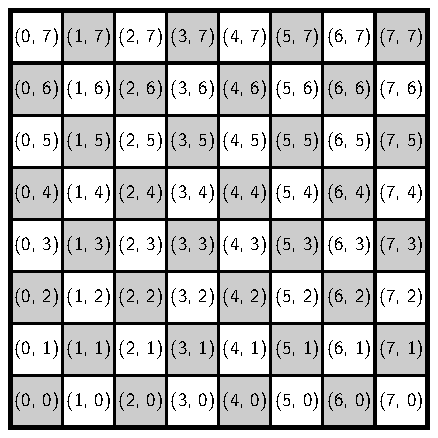
\includegraphics{knight_grid}} \hspace{0.2in} \resizebox{!}{2.3in}{\includegraphics{knight_move_2}}
\caption{Initial knight placement and moves.}
\label{F:knight_2}
\end{center}
\end{figure}
%[trim=left bottom right top, clip]

Each player has two knights to start the game, for one player the knights would begin in positions $(1,0)$ and $(6,0)$. Because of the symmetry of the knight's moves, we will only analyze the moves of the knight that begins at position $(1,0)$. This knight has only three allowable moves from its starting point (assuming that the board is empty), as shown at right in Figure \ref{F:knight_2}. The questions we will ask are: given any position on the board, can the knight move from its start position to that position using only knight moves and, what sequence of moves will make that happen. To answer these questions we will use linear combinations of knight moves described as vectors.

Each knight move can be described by a vector. A move one position to the right and two up can be represented as $\vn_1 = \left[ \begin{array}{c} 1\\2 \end{array} \right]$. Three other moves are $\vn_2 = \left[ \begin{array}{r} -1\\2 \end{array} \right]$, $\vn_3 = \left[ \begin{array}{c} 2\\1 \end{array} \right]$, and $\vn_4 = \left[ \begin{array}{r} -2\\1 \end{array} \right]$. The other four knight moves are the opposites of these four. Any sequence of moves by the knight is given by the linear combination
\[x_1 \vn_1 + x_2 \vn_2 + x_3 \vn_3 + x_4 \vn_4.\]
A word of caution: the knight can only make complete moves, so we are restricted to integer (either positive or negative) values for $x_1$, $x_2$, $x_3$, and $x_4$. You can use the GeoGebra app at \url{https://www.geogebra.org/m/dfwtskrj} to see the effects the weights have on the knight moves.  We should note here that since addition of vectors is commutative, the order in which we apply our moves does not matter. However, we may need to be careful with the order so that our knight does not leave the chess board. 

\begin{pactivity} \label{act:knight_1} ~
\ba
\item Explain why the vector equation 
\[\left[ \begin{array}{c} 1\\0 \end{array} \right] + x_1 \vn_1 + x_2 \vn_2 + x_3 \vn_3 + x_4 \vn_4 = \left[ \begin{array}{c} 5\\2 \end{array} \right]\]
will tell us if it is possible for the knight to move from its initial position at $(1,0)$ to the position (5,2). 

\begin{comment}

A sequence of moves is given by the linear combination $x_1 \vn_1 + x_2 \vn_2 + x_3 \vn_3 + x_4 \vn_4$. Since the knight starts at $(1,0)$, the final position of the knight is 
\[\left[ \begin{array}{c} 1\\0 \end{array} \right] + x_1 \vn_1 + x_2 \vn_2 + x_3 \vn_3 + x_4 \vn_4.\]
So we need to solve the system
\[\left[ \begin{array}{c} 1\\0 \end{array} \right] + x_1 \vn_1 + x_2 \vn_2 + x_3 \vn_3 + x_4 \vn_4 = \left[ \begin{array}{c} 5\\2 \end{array} \right].\]

\end{comment}

	\item Find all solutions, if any, to the system from part (a). If it is possible to find a sequence of moves that take the knight from its initial position to position $(5,2)$, find weights $x_1$, $x_2$, $x_3$, and $x_4$ to accomplish this move. (Be careful -- we must have solutions in which $x_1$, $x_2$, $x_3$, and $x_4$ are integers.) Is there more than one sequence of possible moves? You can check your solution with the GeoGebra app at \url{https://www.geogebra.org/m/dfwtskrj}.

\begin{comment}

The system from part (a) is equivalent to 
\[x_1 \vn_1 + x_2 \vn_2 + x_3 \vn_3 + x_4 \vn_4 = \left[ \begin{array}{c} 4\\2 \end{array} \right].\]
We solve this system by row reducing the augmented matrix
\[\left[ \begin{array}{crcr|c} 1&-1&2&-2&4 \\ 2&2&1&1&2 \end{array} \right].\]
The reduced row echelon form of this matrix is 
\[\left[ \renewcommand{\arraystretch}{1.4} \begin{array}{ccrr|r} 1&0&\frac{5}{4}&-\frac{3}{4}&\frac{5}{2} \\ 0&1&-\frac{3}{4}&\frac{5}{4}&-\frac{3}{2} \end{array} \right].\]
This makes $x_3$ and $x_4 arbitrary, and 
\begin{align*}
x_1 &= -\frac{5}{4}x_3 + \frac{3}{4}x_4 + \frac{5}{2} = \frac{1}{4}\left( -5x_3 + 3x_4 + 10\right) \\
x_2 &= \frac{3}{4}x_3 - \frac{5}{4}x_4 - \frac{3}{2} = \frac{1}{4}\left( 3x_3 - 5x_4 - 6\right).
\end{align*}
In order to have integer values of $x_1$ and $x_2$, we must choose $x_3$ and $x_4$ carefully. If we let $x_3 = x_4 = 1$, then $x_1 = 2$ and $x_2 = -2$. So we can make move $\vn_1$ twice, move $-\vn_2$ twice, and moves $\vn_3$ and $\vn_4$ once each. 

This is not the only possibility. If we let $x_4 = 2$ and $x_3 = 0$, then $x_1 = 4$ and $x_2 = -4$. 

\end{comment}

	\ea
	
\end{pactivity}

Project Activity \ref{act:knight_1} shows that it is possible for our knight to move to position $(5,2)$ on the board. We would like to know if it is possible to move to any position on the board. That is, we would like to know if the span of the four moves $\vn_1$, $\vn_2$, $\vn_3$, and $\vn_4$ will allow our knight to cover the entire board. This takes a bit more work. 

\begin{pactivity} \label{act:knight_2} Given any position $(a,b)$, we want to know if our knight can move from its start position $(1,0)$ to position $(a,b)$. 
	\ba
	\item Write a vector equation whose solution will tell us if it is possible for our knight to move from its start position $(1,0)$ to position $(a,b)$. 

\begin{comment}

As in Project Activity \ref{act:knight_1}, an equation that tells us if this move is possible is
\[\left[ \begin{array}{c} 1\\0 \end{array} \right] + x_1 \vn_1 + x_2 \vn_2 + x_3 \vn_3 + x_4 \vn_4 = \left[ \begin{array}{c} a\\b \end{array} \right],\]
or
\[ x_1 \vn_1 + x_2 \vn_2 + x_3 \vn_3 + x_4 \vn_4 = \left[ \begin{array}{c} a-1\\b \end{array} \right].\]

\end{comment}

	\item Show that the solution to part (a) can be written in the form
	\begin{align}
	x_1 &= \frac{1}{4}\left(-5x_3+3x_4+b+2(a-1)\right) \label{eq:knight_x1} \\
	x_2 &= \frac{1}{4}\left(3x_3-5x_4+b-2(a-1)\right) \label{eq:knight_x2} \\
	x_3 &\text{ is free} \notag \\
	x_4 &\text{ is free.} \notag
	\end{align}

\begin{comment}

Using technology we see that the reduced row echelon form of 
\[\left[ \begin{array}{crcr|c} 1&-1&2&-2&a-1 \\ 2&2&1&1&b \end{array} \right]\]
is 
\[\left[ \renewcommand{\arraystretch}{1.4} \begin{array}{ccrr|r} 1&0&\frac{5}{4}&-\frac{3}{4}&\frac{1}{4}(b+2(a-1)) \\ 0&1&-\frac{3}{4}&\frac{5}{4}&\frac{1}{4}(b-2(a-1)) \end{array} \right].\]
This makes $x_3$ and $x_4 free, and 
\begin{align*}
x_1 &= -\frac{5}{4}x_3 + \frac{3}{4}x_4 + \frac{1}{4}(b+2(a-1)) = \frac{1}{4}\left( -5x_3 + 3x_4 + b + 2(a-1)\right) \\
x_2 &= \frac{3}{4}x_3 - \frac{5}{4}x_4 + \frac{1}{4}(b-2(a-1)) = \frac{1}{4}\left( 3x_3 - 5x_4 + b - 2(a-1) \right).
\end{align*}

\end{comment}

	\ea
\end{pactivity}

To answer our question if our knight can reach any position, we now need to determine if we can always find integer values of $x_3$ and $x_4$ to make equations (\ref{eq:knight_x1}) and (\ref{eq:knight_x2}) have integer solutions. In other words, we need to find values of $x_3$ and $x_4$ so that $-5x_3+3x_4+b+2(a-1)$ and $3x_3-5x_4+b-2(a-1)$ are multiples of $4$. How we do this could depend on the parity (even or odd) of $a$ and $b$. For example, if $a$ is odd and $b$ is even, say $a = 2r+1$ and $b = 2s$ for some integers $r$ and $s$, then
\begin{align*}
x_1 &= \frac{1}{4}\left( -5x_3 + 3x_4 + 2s + 4r\right) \\
x_2 &= \frac{1}{4}\left( 3x_3 - 5x_4 + 2s - 4r \right).
\end{align*}
With a little trial and error we can see that if we let $x_3 = x_4 = s$, then $x_1 = r$ and $x_2 = -r$ is a solution with integer weights. For example, when $a=5$ and $b=2$ we have $r=2$ and $s = 1$. This makes $x_1 = 2$, $x_2 = -2$, $x_3 = 1 = x_4$. Compare this to the solution(s) you found in Project Activity \ref{act:knight_1}. This analysis shows us how to move our knight to any position $(a,b)$ where $a$ is odd and $b$ is even.

\begin{pactivity} \label{act:knight_3} Complete the analysis as above to determine if there are integer solutions to our knight's move system in the following cases.
	\ba
	\item $a$ odd and $b$ odd
	\item $a$ even and $b$ even
	\item $a$ even and $b$ odd.
	\ea

\begin{comment}

\ba
\item Assume that $a$ is odd and $b$ is odd. That is, $a = 2r+1$ and $b = 2s+1$ for some integers $r$ and $s$. Then
\begin{align*}
x_1 &= \frac{1}{4}\left( -5x_3 + 3x_4 + 2s + 1 + 4r\right) \\
x_2 &= \frac{1}{4}\left( 3x_3 - 5x_4 + 2s + 1 - 4r \right).
\end{align*}
With a little trial and error we can see that if we let $x_3 = 2s+1$ and $x_4 = 0$, then $x_1 = -2s+r-1$ and $x_2 = 2s-r+1$ is a solution with integer weights. 

\item Assume that $a$ is even and $b$ is even. That is, $a = 2r$ and $b = 2s$ for some integers $r$ and $s$. Then
\begin{align*}
x_1 &= \frac{1}{4}\left( -5x_3 + 3x_4 + 2s  + 4r - 2\right) \\
x_2 &= \frac{1}{4}\left( 3x_3 - 5x_4 + 2s + 1 - 4r + 2 \right).
\end{align*}
With a little trial and error we can see that if we let $x_3 = 2s+1$ and $x_4 = 1$, then $x_1 = -2s+r-1$ and $x_2 = 2s-r$ is a solution with integer weights. 

\item Assume that $a$ is even and $b$ is odd. That is, $a = 2r$ and $b = 2s+1$ for some integers $r$ and $s$. Then
\begin{align*}
x_1 &= \frac{1}{4}\left( -5x_3 + 3x_4 + 2s - 1 + 4r\right) \\
x_2 &= \frac{1}{4}\left( 3x_3 - 5x_4 + 2s + 3 - 4r \right).
\end{align*}
With a little trial and error we can see that if we let $x_3 = 2s$ and $x_4 = -1$, then $x_1 = -2s+r-1$ and $x_2 = 2s-r+2$ is a solution with integer weights. 
\ea

\end{comment}

\end{pactivity}

Project Activity \ref{act:knight_3} shows that for any position on the chess board, using linear combinations of move vectors, we can find a sequence of moves that takes our knight to that position. (We actually haven't shown that these moves can be made so that our knight always stays on the board -- we leave that question to you.)

